% Editable native annotations around unchanged verified IDE photographs.
\par
\begin{figure}[htbp]
\centering
\newsavebox{\MARSfirimpulseregistersBox}
\sbox{\MARSfirimpulseregistersBox}{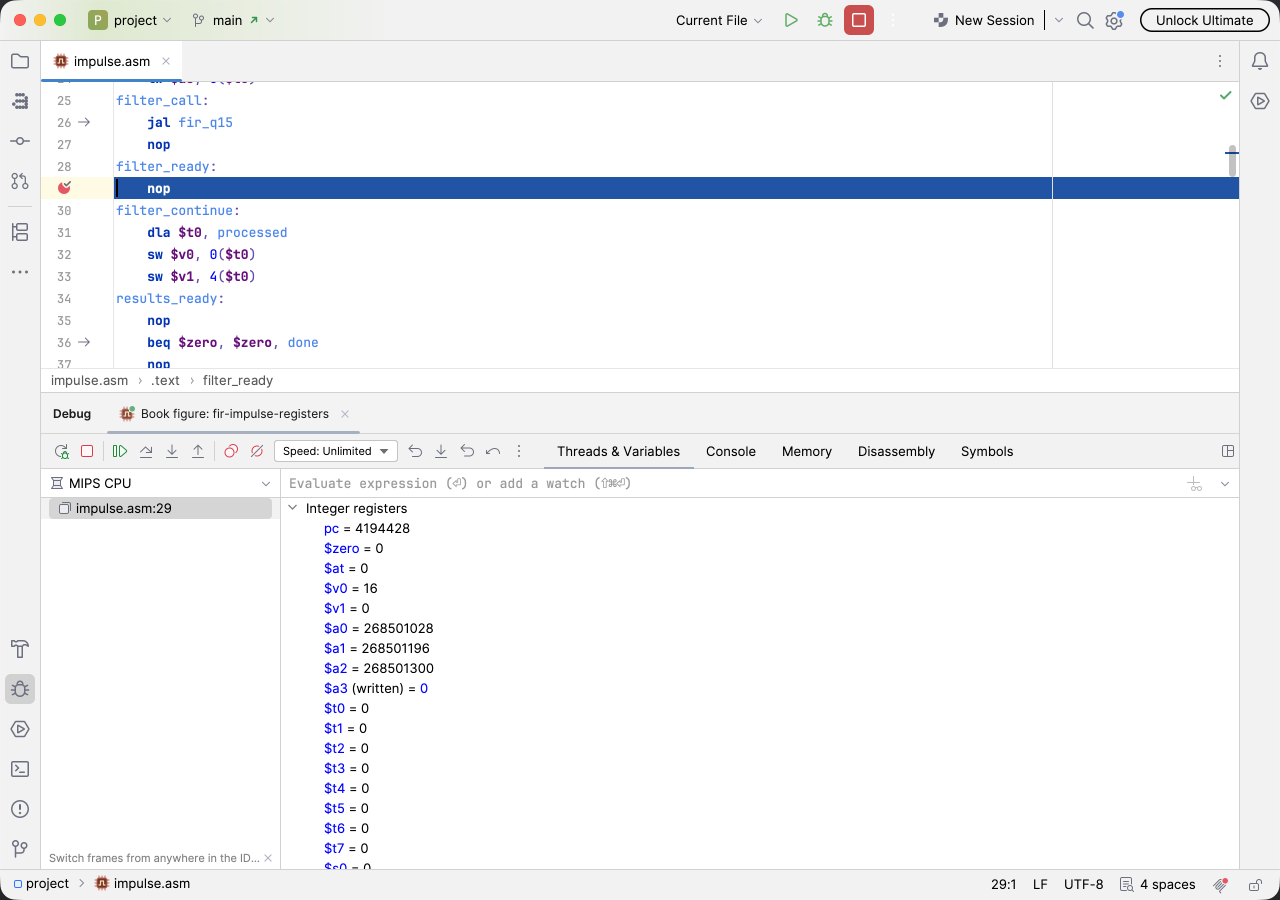
\includegraphics[artifact]{packages/021-fixed-point-fir/captures/f01/registers.png}}
\newsavebox{\MARSfirimpulseinputBox}
\sbox{\MARSfirimpulseinputBox}{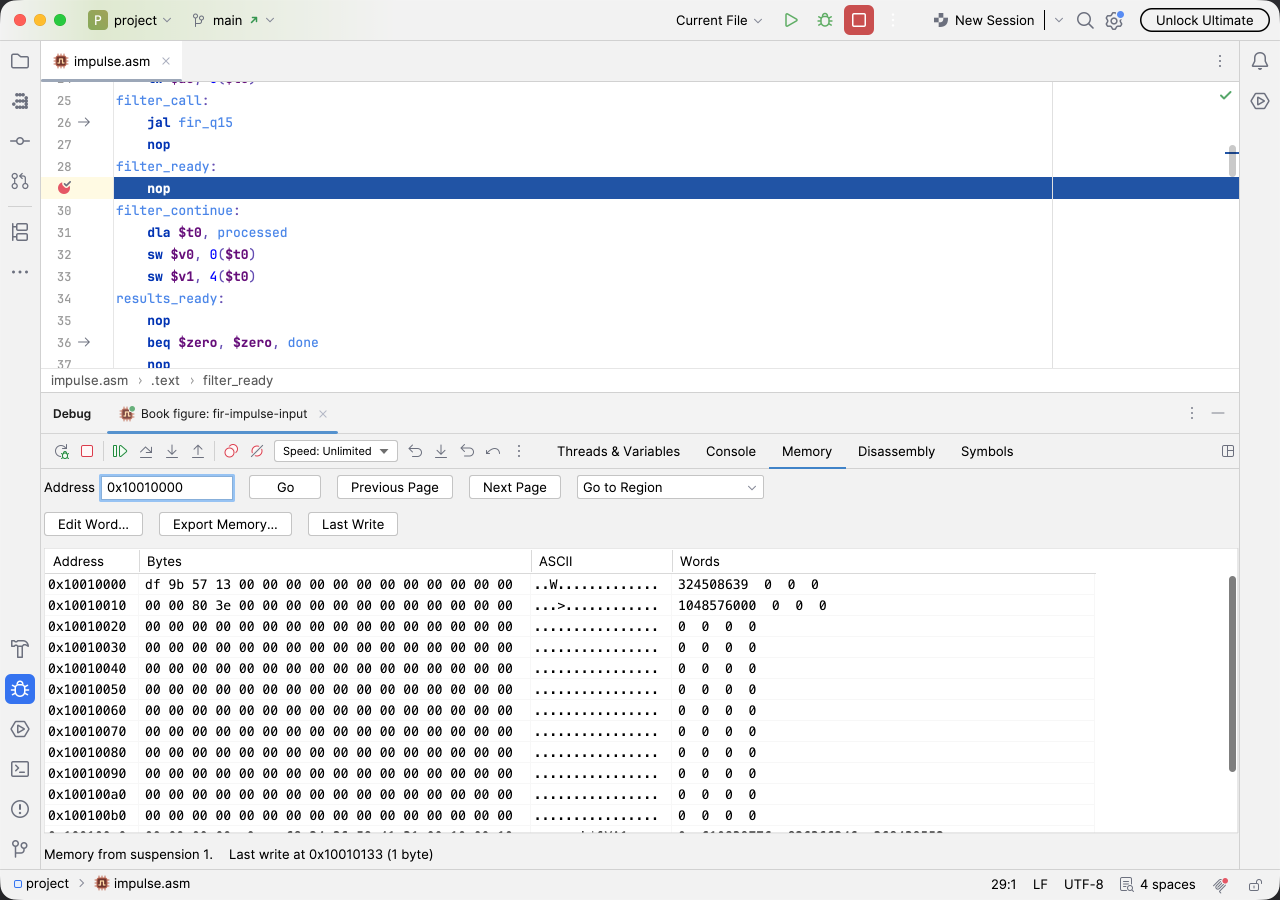
\includegraphics[artifact]{packages/021-fixed-point-fir/captures/f01/input.png}}
\newsavebox{\MARSfirimpulsecoefficientsBox}
\sbox{\MARSfirimpulsecoefficientsBox}{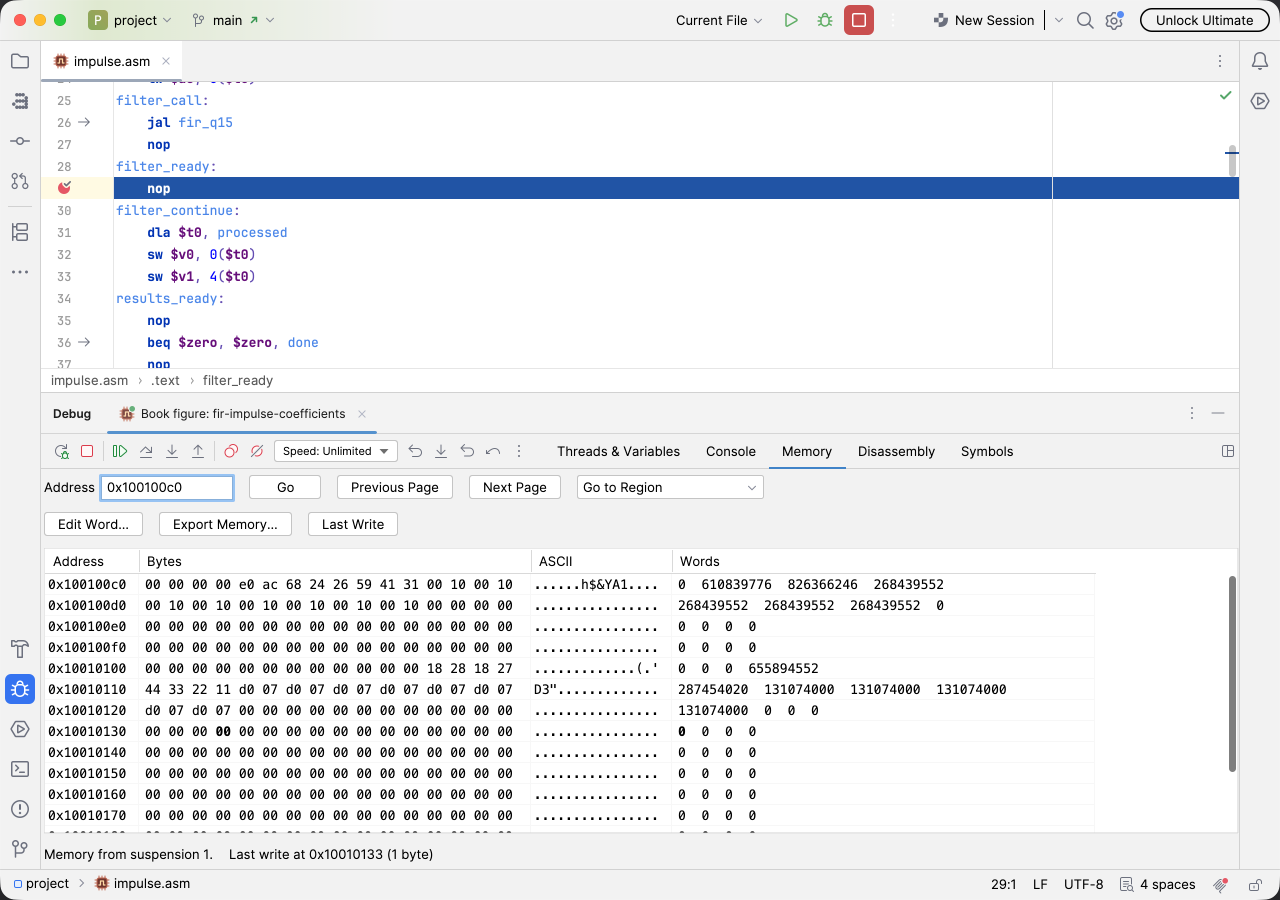
\includegraphics[artifact]{packages/021-fixed-point-fir/captures/f01/coefficients.png}}
\newsavebox{\MARSfirimpulseoutputBox}
\sbox{\MARSfirimpulseoutputBox}{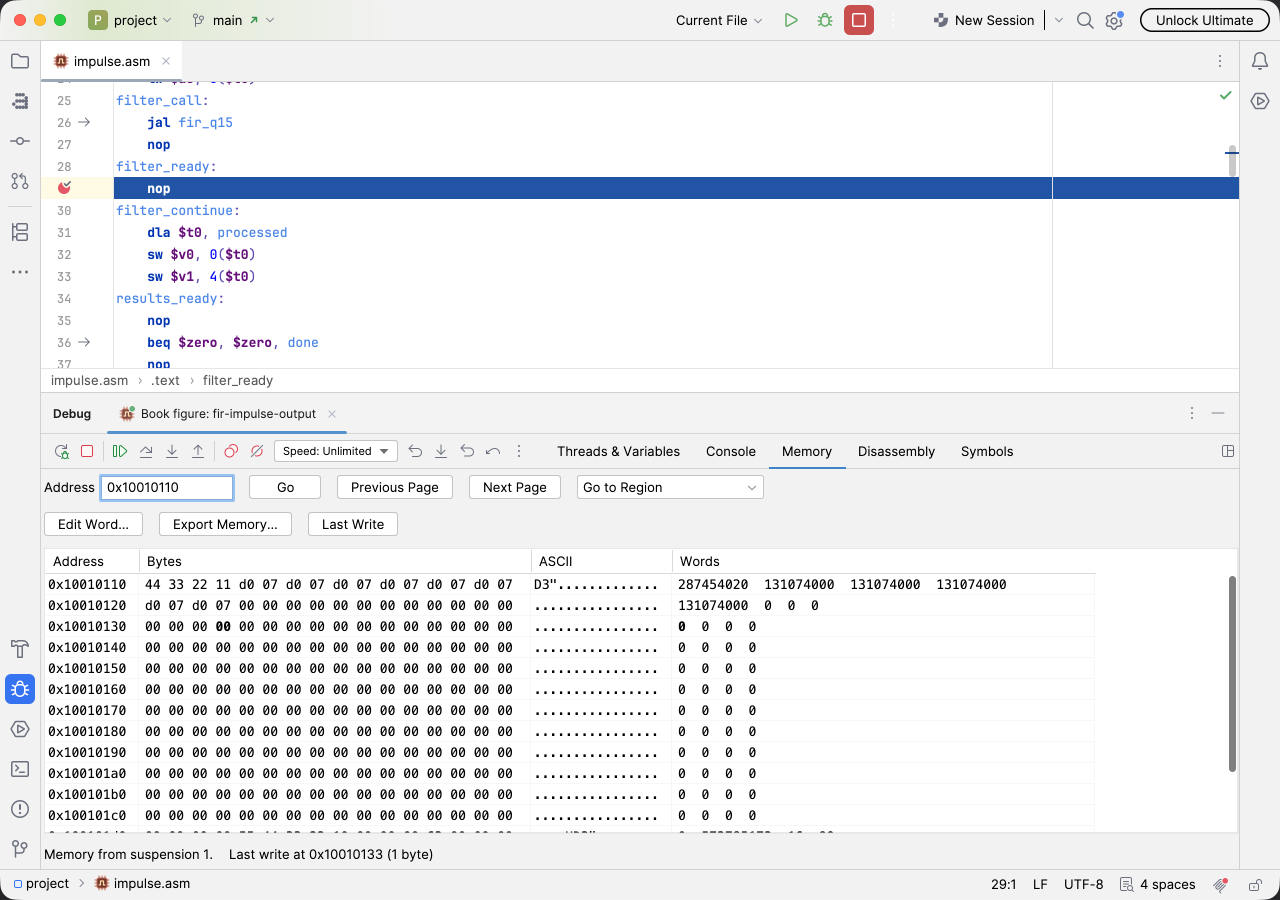
\includegraphics[artifact]{packages/021-fixed-point-fir/captures/f01/output.png}}
\newsavebox{\MARSfirimpulsecallerBox}
\sbox{\MARSfirimpulsecallerBox}{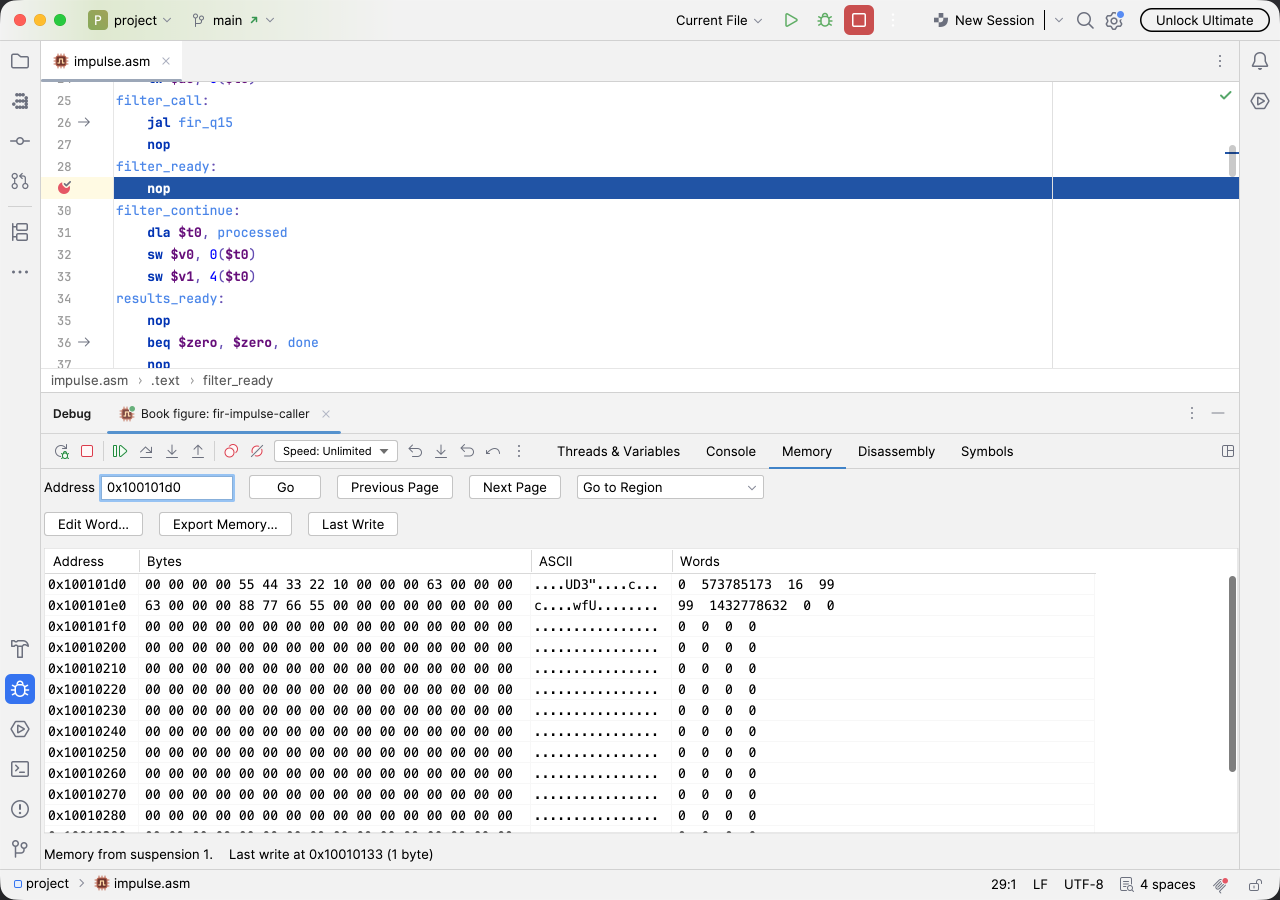
\includegraphics[artifact]{packages/021-fixed-point-fir/captures/f01/caller.png}}
\edef\MARSfirimpulsesourceLeft{\the\dimexpr0.036718750\wd\MARSfirimpulseregistersBox\relax}
\edef\MARSfirimpulsesourceBottom{\the\dimexpr0.774444444\ht\MARSfirimpulseregistersBox\relax}
\edef\MARSfirimpulsesourceRight{\the\dimexpr0.713281250\wd\MARSfirimpulseregistersBox\relax}
\edef\MARSfirimpulsesourceTop{\the\dimexpr0.170000000\ht\MARSfirimpulseregistersBox\relax}
\edef\MARSfirimpulseregistersLeft{\the\dimexpr0.246093750\wd\MARSfirimpulseregistersBox\relax}
\edef\MARSfirimpulseregistersBottom{\the\dimexpr0.312222222\ht\MARSfirimpulseregistersBox\relax}
\edef\MARSfirimpulseregistersRight{\the\dimexpr0.553906250\wd\MARSfirimpulseregistersBox\relax}
\edef\MARSfirimpulseregistersTop{\the\dimexpr0.640000000\ht\MARSfirimpulseregistersBox\relax}
\edef\MARSfirimpulseinputLeft{\the\dimexpr0.034375000\wd\MARSfirimpulseinputBox\relax}
\edef\MARSfirimpulseinputBottom{\the\dimexpr0.311111111\ht\MARSfirimpulseinputBox\relax}
\edef\MARSfirimpulseinputRight{\the\dimexpr0.584375000\wd\MARSfirimpulseinputBox\relax}
\edef\MARSfirimpulseinputTop{\the\dimexpr0.608888889\ht\MARSfirimpulseinputBox\relax}
\edef\MARSfirimpulsecoefficientsLeft{\the\dimexpr0.034375000\wd\MARSfirimpulsecoefficientsBox\relax}
\edef\MARSfirimpulsecoefficientsBottom{\the\dimexpr0.311111111\ht\MARSfirimpulsecoefficientsBox\relax}
\edef\MARSfirimpulsecoefficientsRight{\the\dimexpr0.584375000\wd\MARSfirimpulsecoefficientsBox\relax}
\edef\MARSfirimpulsecoefficientsTop{\the\dimexpr0.608888889\ht\MARSfirimpulsecoefficientsBox\relax}
\edef\MARSfirimpulseoutputLeft{\the\dimexpr0.034375000\wd\MARSfirimpulseoutputBox\relax}
\edef\MARSfirimpulseoutputBottom{\the\dimexpr0.311111111\ht\MARSfirimpulseoutputBox\relax}
\edef\MARSfirimpulseoutputRight{\the\dimexpr0.584375000\wd\MARSfirimpulseoutputBox\relax}
\edef\MARSfirimpulseoutputTop{\the\dimexpr0.608888889\ht\MARSfirimpulseoutputBox\relax}
\edef\MARSfirimpulsecallerLeft{\the\dimexpr0.034375000\wd\MARSfirimpulsecallerBox\relax}
\edef\MARSfirimpulsecallerBottom{\the\dimexpr0.311111111\ht\MARSfirimpulsecallerBox\relax}
\edef\MARSfirimpulsecallerRight{\the\dimexpr0.584375000\wd\MARSfirimpulsecallerBox\relax}
\edef\MARSfirimpulsecallerTop{\the\dimexpr0.608888889\ht\MARSfirimpulsecallerBox\relax}
\begin{tikzpicture}[alt={Six annotated panels at filter_ready show returns sixteen and zero. Seven zero history samples precede an impulse of 16000. Eight coefficient codes of 4096 produce eight output codes of 2000 followed by zeros. Caller processed and clipped remain 99, while all input and coefficient bytes are unchanged.}]
\node[anchor=north west,inner sep=0,font=\small\bfseries] (source-title) at (6mm,0) {Next instruction at this boundary};
\node[anchor=north west,inner sep=0] (source) at ([yshift=-1mm]source-title.south west) {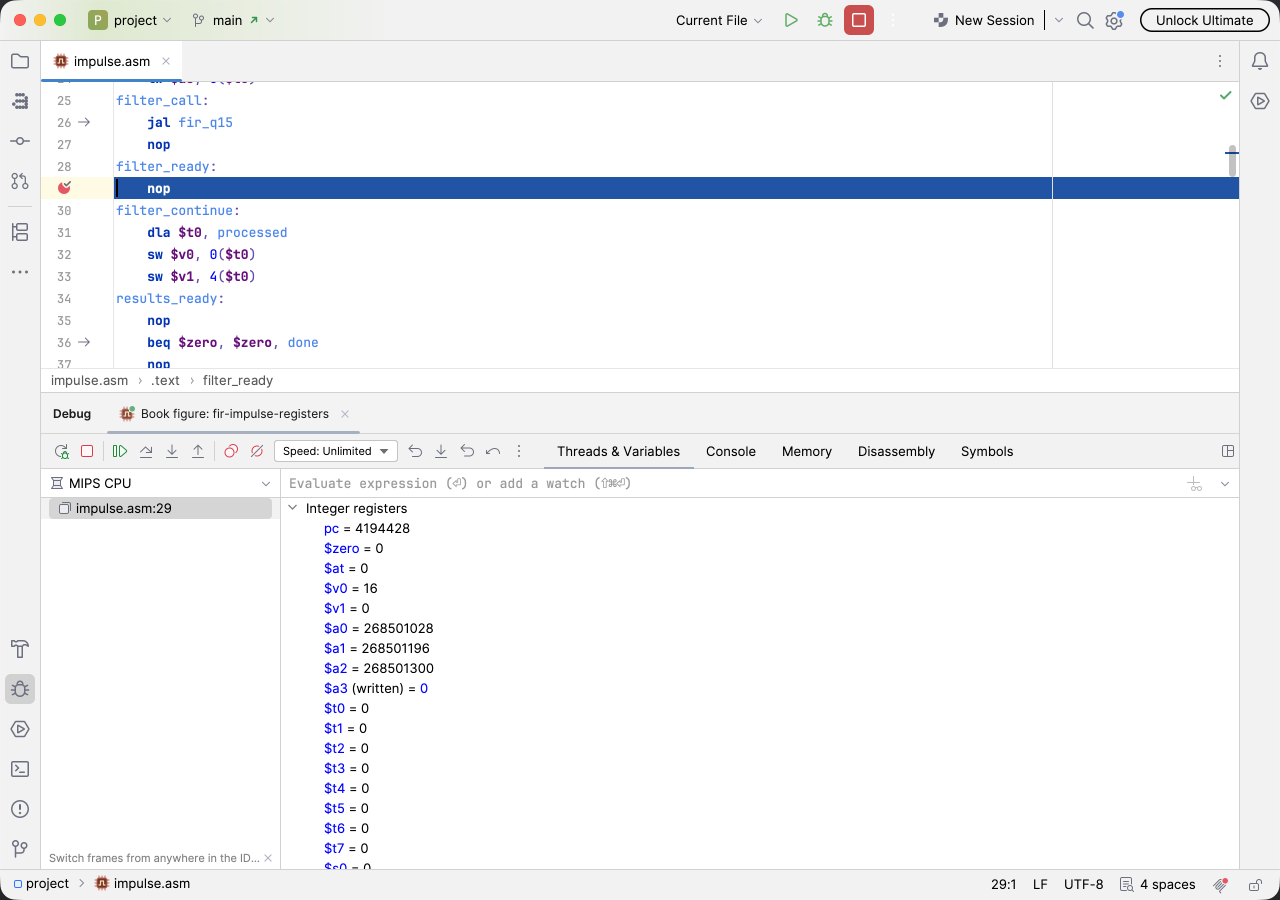
\includegraphics[width=0.54\linewidth,artifact,trim={\MARSfirimpulsesourceLeft{} \MARSfirimpulsesourceBottom{} \MARSfirimpulsesourceRight{} \MARSfirimpulsesourceTop{}},clip]{packages/021-fixed-point-fir/captures/f01/registers.png}};
\begin{scope}[shift={(source.south west)},x={($(source.south east)-(source.south west)$)},y={($(source.north west)-(source.south west)$)}]
\draw[black,line width=0.7pt] (0.215625000,0.080000000) rectangle (0.384375000,0.520000000);
\node[draw=black,fill=white,circle,inner sep=1.5pt,font=\footnotesize] at ($(0.215625000,0.520000000)+(-3mm,0)$) {1};
\end{scope}
\node[anchor=north west,inner sep=0,font=\small\bfseries] (registers-title) at (0.58\linewidth,0 |- source-title.north) {Register values at this boundary};
\node[anchor=north west,inner sep=0] (registers) at ([yshift=-1mm]registers-title.south west) {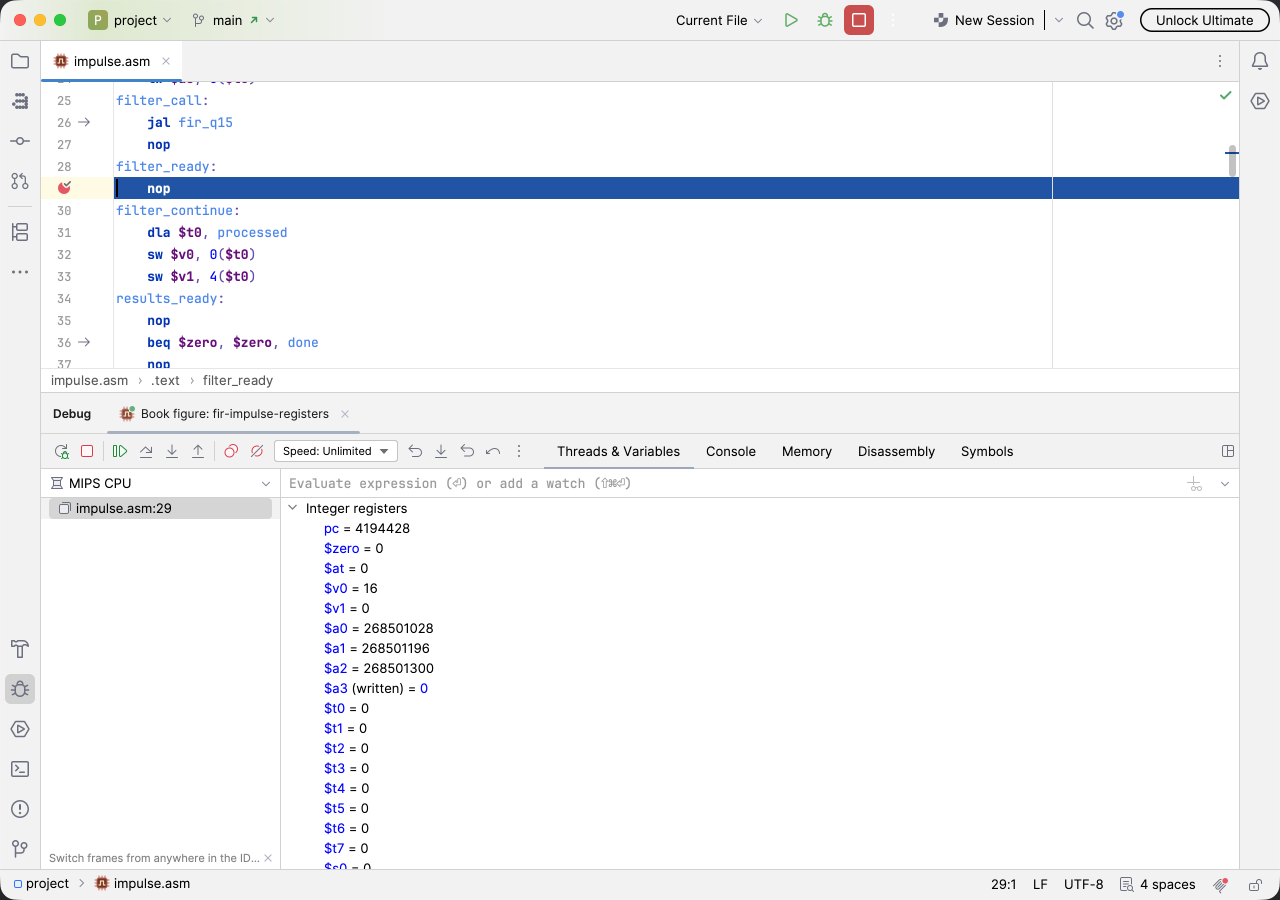
\includegraphics[width=0.42\linewidth,artifact,trim={\MARSfirimpulseregistersLeft{} \MARSfirimpulseregistersBottom{} \MARSfirimpulseregistersRight{} \MARSfirimpulseregistersTop{}},clip]{packages/021-fixed-point-fir/captures/f01/registers.png}};
\begin{scope}[shift={(registers.south west)},x={($(registers.south east)-(registers.south west)$)},y={($(registers.north west)-(registers.south west)$)}]
\draw[black,line width=0.7pt] (0.023437500,0.023255814) rectangle (0.250000000,0.953488372);
\node[draw=black,fill=white,circle,inner sep=1.5pt,font=\footnotesize] at ($(0.023437500,0.953488372)+(-3mm,0)$) {2};
\end{scope}
\node[anchor=north west,inner sep=0,font=\small\bfseries] (input-title) at ([yshift=-1mm]source.south west) {Input window detail};
\node[anchor=north west,inner sep=0] (input) at ([yshift=-1mm]input-title.south west) {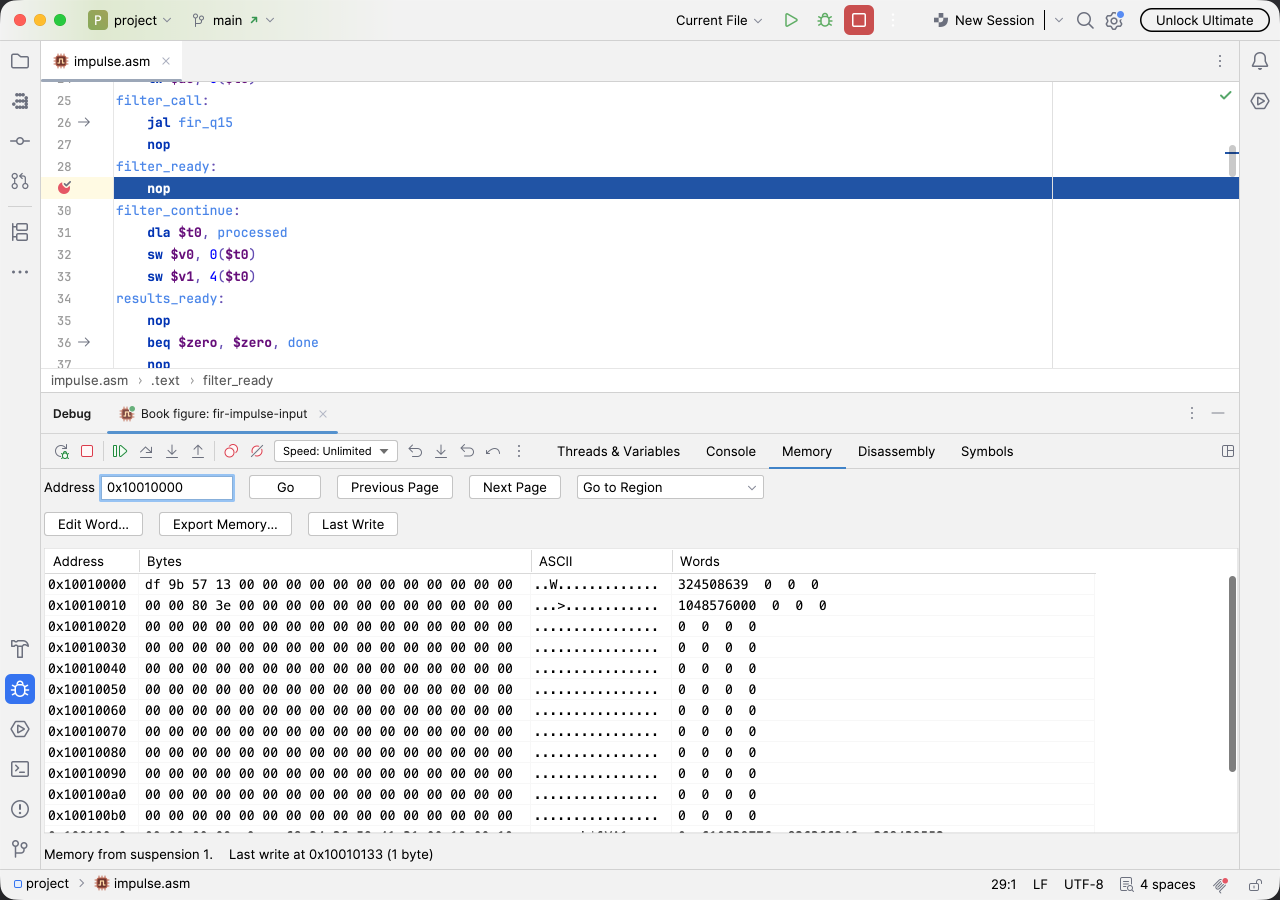
\includegraphics[width=0.84\linewidth,artifact,trim={\MARSfirimpulseinputLeft{} \MARSfirimpulseinputBottom{} \MARSfirimpulseinputRight{} \MARSfirimpulseinputTop{}},clip]{packages/021-fixed-point-fir/captures/f01/input.png}};
\begin{scope}[shift={(input.south west)},x={($(input.south east)-(input.south west)$)},y={($(input.north west)-(input.south west)$)}]
\draw[black,line width=0.7pt] (0.194672131,0.055555556) rectangle (0.997950820,0.638888889);
\node[draw=black,fill=white,circle,inner sep=1.5pt,font=\footnotesize] at ($(0,0.638888889)+(-3mm,0)$) {3};
\end{scope}
\node[anchor=north west,inner sep=0,font=\small\bfseries] (coefficients-title) at ([yshift=-1mm]input.south west) {Eight signed coefficient codes};
\node[anchor=north west,inner sep=0] (coefficients) at ([yshift=-1mm]coefficients-title.south west) {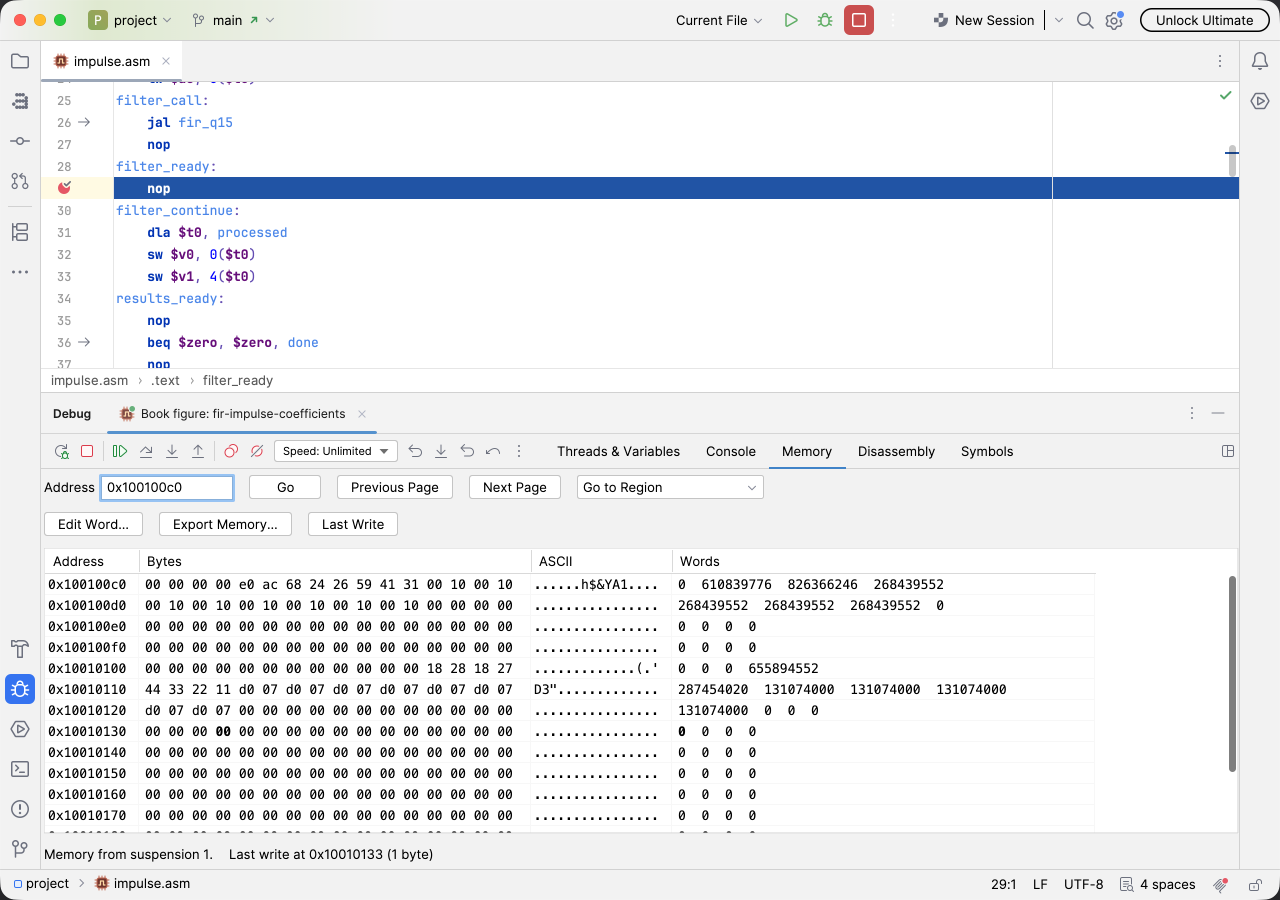
\includegraphics[width=0.84\linewidth,artifact,trim={\MARSfirimpulsecoefficientsLeft{} \MARSfirimpulsecoefficientsBottom{} \MARSfirimpulsecoefficientsRight{} \MARSfirimpulsecoefficientsTop{}},clip]{packages/021-fixed-point-fir/captures/f01/coefficients.png}};
\begin{scope}[shift={(coefficients.south west)},x={($(coefficients.south east)-(coefficients.south west)$)},y={($(coefficients.north west)-(coefficients.south west)$)}]
\draw[black,line width=0.7pt] (0.194672131,0.055555556) rectangle (0.997950820,0.638888889);
\node[draw=black,fill=white,circle,inner sep=1.5pt,font=\footnotesize] at ($(0,0.638888889)+(-3mm,0)$) {4};
\end{scope}
\node[anchor=north west,inner sep=0,font=\small\bfseries] (output-title) at ([yshift=-1mm]coefficients.south west) {Selected output halfwords};
\node[anchor=north west,inner sep=0] (output) at ([yshift=-1mm]output-title.south west) {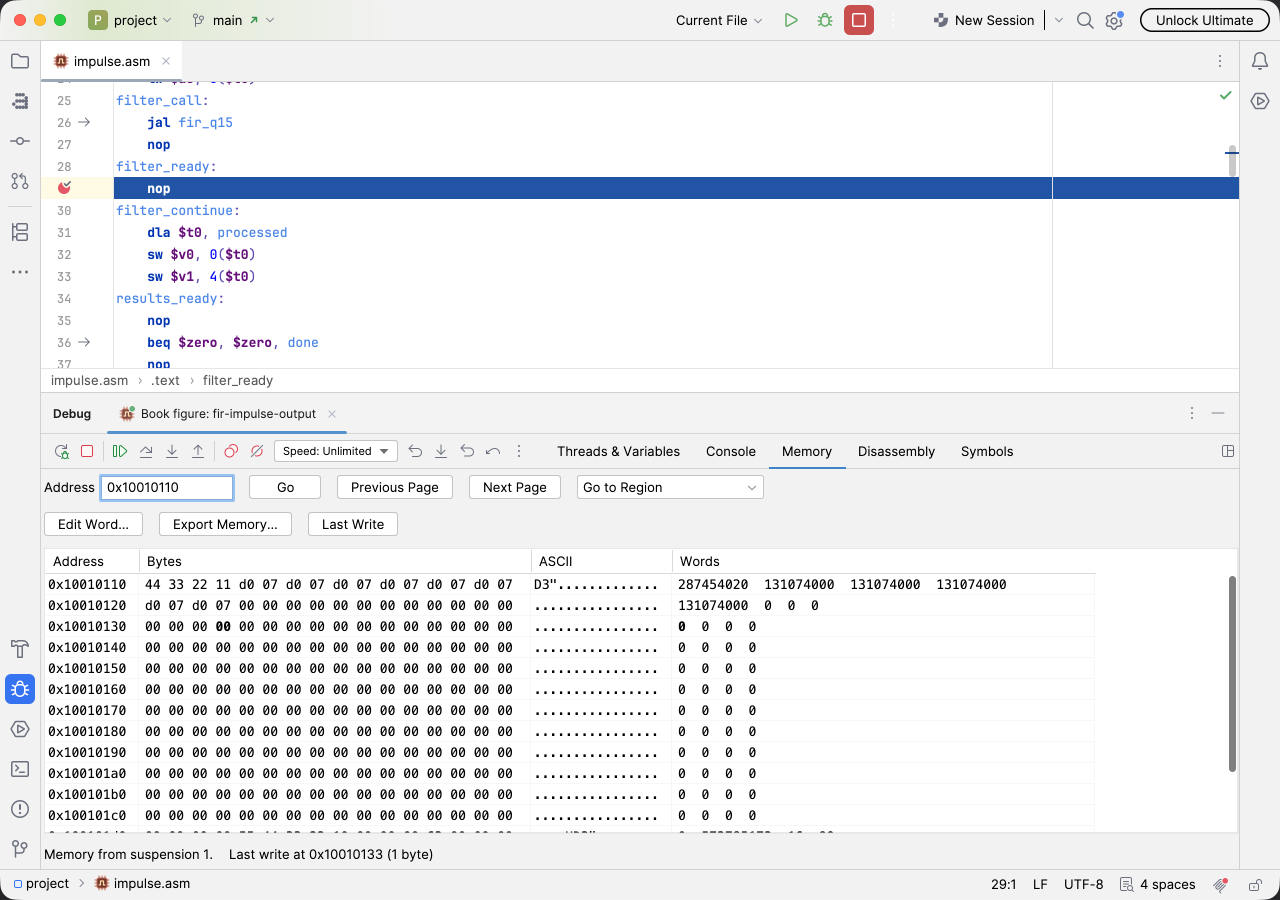
\includegraphics[width=0.84\linewidth,artifact,trim={\MARSfirimpulseoutputLeft{} \MARSfirimpulseoutputBottom{} \MARSfirimpulseoutputRight{} \MARSfirimpulseoutputTop{}},clip]{packages/021-fixed-point-fir/captures/f01/output.png}};
\begin{scope}[shift={(output.south west)},x={($(output.south east)-(output.south west)$)},y={($(output.north west)-(output.south west)$)}]
\draw[black,line width=0.7pt] (0.194672131,0.055555556) rectangle (0.997950820,0.638888889);
\node[draw=black,fill=white,circle,inner sep=1.5pt,font=\footnotesize] at ($(0,0.638888889)+(-3mm,0)$) {5};
\end{scope}
\node[anchor=north west,inner sep=0,font=\small\bfseries] (caller-title) at ([yshift=-1mm]output.south west) {Count and saved caller results};
\node[anchor=north west,inner sep=0] (caller) at ([yshift=-1mm]caller-title.south west) {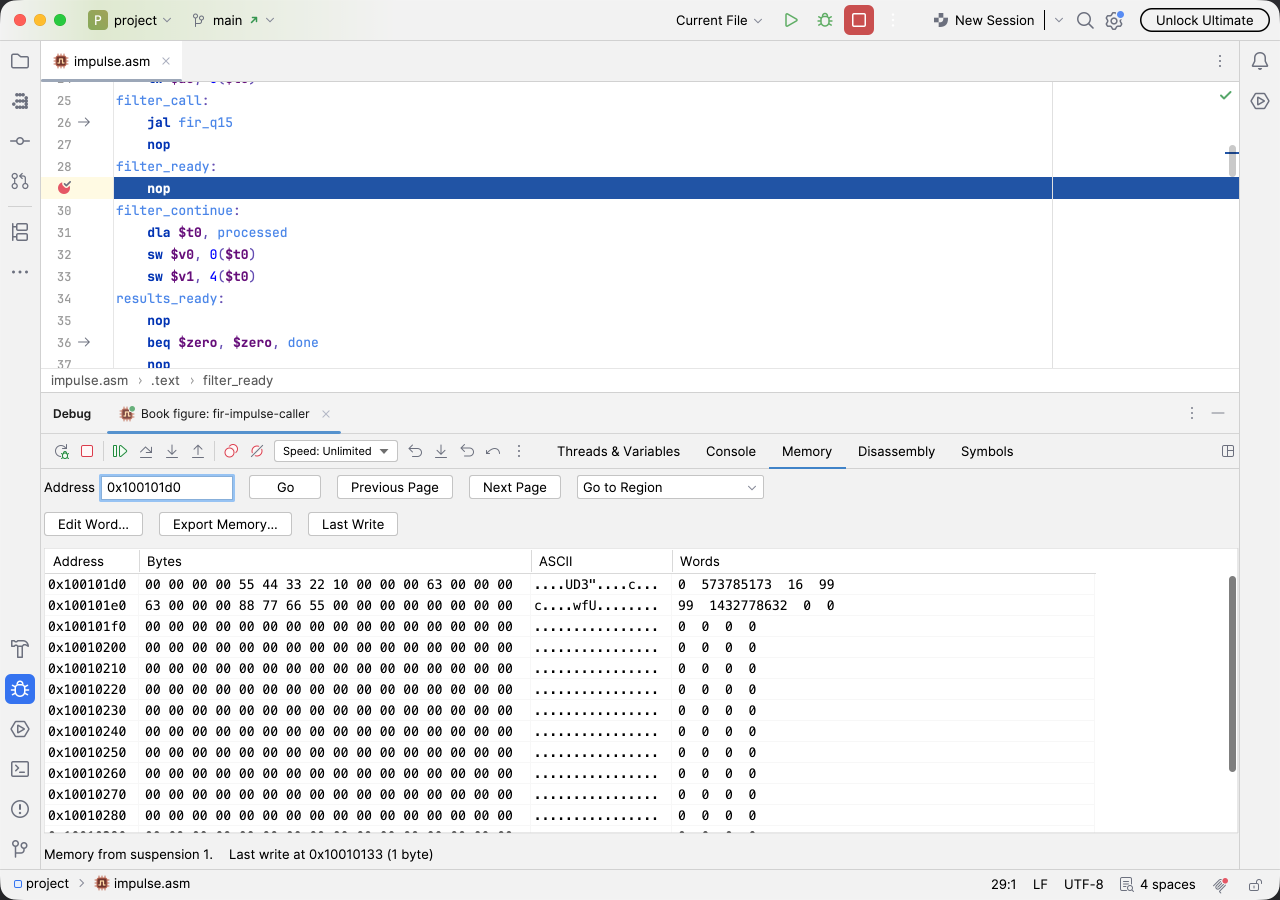
\includegraphics[width=0.84\linewidth,artifact,trim={\MARSfirimpulsecallerLeft{} \MARSfirimpulsecallerBottom{} \MARSfirimpulsecallerRight{} \MARSfirimpulsecallerTop{}},clip]{packages/021-fixed-point-fir/captures/f01/caller.png}};
\begin{scope}[shift={(caller.south west)},x={($(caller.south east)-(caller.south west)$)},y={($(caller.north west)-(caller.south west)$)}]
\draw[black,line width=0.7pt] (0.194672131,0.055555556) rectangle (0.997950820,0.638888889);
\node[draw=black,fill=white,circle,inner sep=1.5pt,font=\footnotesize] at ($(0,0.638888889)+(-3mm,0)$) {6};
\end{scope}
\end{tikzpicture}
\par\smallskip
\begin{minipage}{\linewidth}
\small
\begin{enumerate}
\setlength{\itemsep}{2pt}
\setlength{\parsep}{0pt}
\item The blue \texttt{nop} at \texttt{filter\_ready} follows the filtering return. The output is complete, but the caller has not yet copied the two result registers into \texttt{processed} and \texttt{clipped}.
\item \texttt{\$v0 = 16} counts outputs and \texttt{\$v1 = 0} counts rounded values requiring saturation. Sixteen outputs require 23 input samples: seven history samples followed by sixteen new samples.
\item Input begins at \texttt{0x10010004}, after its guard. The seven history samples are zero. Bytes \texttt{80 3e} at \texttt{0x10010012} encode the newest sample of the first window, 16000. Each later window advances by one halfword.
\item The eight coefficients begin at \texttt{0x100100cc}. Each code is 4096 (\texttt{00 10}), representing $1/8$. The impulse contributes $16000\cdot4096=65536000$ to each window that contains it.
\item Output begins at \texttt{0x10010114}. Each of the first eight results is 2000, stored as \texttt{d0 07}; later results are zero. As the window advances, the impulse moves through all eight tap positions and then leaves the window.
\item The caller count is 16. The two saved result words still contain 99 (\texttt{63 00 00 00}), because their stores follow this stop. Source, coefficient and output suffixes are preserved.
\end{enumerate}
\end{minipage}
\caption{The sixteen-output impulse call returns before its result words are stored.}
\label{capture:021-fixed-point-fir-f01}
\label{fir-f01}
\end{figure}
\par
